%#! pdflatex
%
% $Id: manual.tex,v 1.36 2022/12/05 06:59:50 tanaka Rel tanaka $
% $Revision: 1.36 $
% $Date: 2022/12/05 06:59:50 $
% $Author: tanaka $
%
\documentclass[a4paper]{book}
\usepackage{graphicx}
\usepackage{fancybox}
\usepackage{color}
\usepackage[%bookmarks=true,bookmarksnumbered=true,
 pdftitle={SiPS/SiPSi User Guide},%
 pdfauthor={Shunji Tanaka},%
 colorlinks=true,%
 linktocpage=true]{hyperref}
\newenvironment{fminipage}%
{\begin{Sbox}\begin{minipage}}{\end{minipage}\end{Sbox}\fbox{\TheSbox}}
\newenvironment{xminipage}%
{\begin{center}\begin{Sbox}\begin{minipage}{0.96\textwidth}\mbox{}\\[-15pt]}%
{\mbox{}\\[-21pt]\end{minipage}\end{Sbox}\fbox{\TheSbox}\end{center}}
\newcounter{lineno}
\newenvironment{listing}[1]%
{\begin{list}{\arabic{lineno}:}{\usecounter{lineno}%
   \setcounter{lineno}{#1}%
   \addtocounter{lineno}{-1}%
   \setlength{\baselineskip}{10pt}%
   \setlength{\itemindent}{-5pt}%
   \setlength{\labelwidth}{22pt}%
   \setlength{\parsep}{0pt}}}%
{\end{list}}

\begin{document}
\title{SiPS/SiPSi Version 1.08p4 Reference Manual}
\author{Shunji Tanaka}
\date{Dec 6, 2022}
\maketitle

\tableofcontents

\chapter{Introduction}

SiPS (\underline{Si}ngle-machine scheduling \underline{P}roblem \underline{S}olver) and SiPSi (\underline{Si}ngle-machine scheduling \underline{P}roblem \underline{S}olver with \underline{i}dle time) are solvers for general single-machine scheduling to minimize total job completion cost.
They are currently offered as C libraries.
For the detailed algorithms, please refer to our paper:

\begin{quotation}
  S.~Tanaka, S.~Fujikuma, and M.~Araki (2009).
  An exact algorithm for single-machine scheduling without machine idle time,
  Journal of Scheduling, vol.~12, no.~6, pp.~575--593.
  \href{http://dx.doi.org/10.1007/s10951-008-0093-5}%
  {DOI:10.1007/s10951-008-0093-5}.

  S.~Tanaka and S.~Fujikuma (2012).
  A dynamic-programming-based exact algorithm for general
  single-machine scheduling with machine idle time,
  Journal of Scheduling. vol.~15, no.~3, pp.~347--361.
  \href{http://dx.doi.org/10.1007/s10951-011-0242-0}%
  {DOI:10.1007/s10951-011-0242-0}.
\end{quotation}

SiPS/SiPSi is distributed under the {\bf 2-clause BSD license}.
It is not a license condition, but I am pleased if you will refer to the above papers when you write a paper using SiPS/SiPSi because the \href{https://sites.google.com/site/shunjitanaka/sips}{URL} offering the program may change in the future. Also, donation is welcome. ;-)

My contact address is
\begin{quote}
  Shunji Tanaka\\
  Department of Electrical Engineering, Kyoto University\\
  Kyotodaigaku-Katsura, Nishikyo-ku, Kyoto 615-8510, Japan\\
  \href{mailto:tanaka@kuee.kyoto-u.ac.jp}{tanaka@kuee.kyoto-u.ac.jp}
\end{quote}

\section{Single-Machine Scheduling Problem}

Consider that $n$ jobs (job $1$, job $2$, $\ldots$, job $n$) are to be processed on a single machine.
Each job $i\in\mathcal{N}=\{1,2,\ldots,n\}$ is given an integer processing time $p_i$, an integer release date $r_i$ and a cost function $f_i(t)$.
The machine can process at most one job at a time and no preemption is allowed.
Denote the completion time of job $i$ by $C_i(\ge r_i+p_i)$ and assume that $C_i$ is integral.
The objective is to find a schedule that minimizes the total job completion cost $\sum_{i\in\mathcal{N}}f_i(C_i)$.
According to the standard classification, this problem is referred to as $1||\sum f_i(C_i)$ when $r_i=0$ for all $i\in\mathcal{N}$, or otherwise $1|r_i|\sum f_i(C_i)$.

A schedule is often denoted by a Gantt chart, whose horizontal axis represents the the elapsed time. A simple example is shown in Figure~\ref{fig:Gantt}.

\begin{figure}[tp]
  \centering
  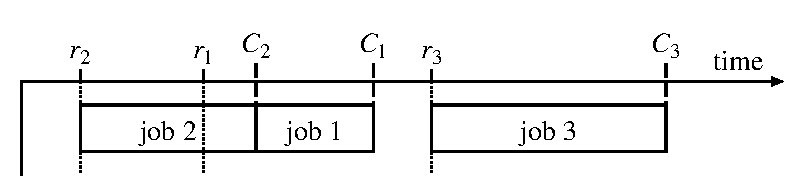
\includegraphics[scale=0.8]{gantt.eps}
  \caption{Gantt Chart of a Schedule}
  \label{fig:Gantt}
\end{figure}


SiPSi is applicable to $1||\sum f_i(C_i)$ and $1|r_i|\sum f_i(C_i)$.
On the other hand, SiPS is only to the problem without idle time, i.e. $1||\sum f_i(C_i)$ without idle time, which is denoted by $1|\mathrm{noidle}|\sum f_i(C_i)$.

Ordinary, the cost function $f_i(t)$ is specified by the 3-tuple ($d_i$, $\alpha_i$, $\beta_i$): an integer due date $d_i$, an earliness weight $\alpha_i$ and
a tardiness weight $\beta_i$.
More specifically, the cost function $f_i(t)$ is given by
\begin{eqnarray}
  f_i(t)
    &=&\alpha_i\max\{d_i-C_i,0\}+\beta_i\max\{C_i-d_i,0\}
    \nonumber\\
    &=&\max\{\alpha_i(d_i-C_i),\beta_i(C_i-d_i)\}.
\end{eqnarray}
Therefore, if ($d_i$, $\alpha_i$, $\beta_i$)$=$($0$, $0$, $w_i$), the objective function becomes the total weighted completion time $\sum_{i\in\mathcal{N}}w_iC_i$ and if ($d_i$, $\alpha_i$, $\beta_i$)$=$($d_i$, $0$, $w_i$), it becomes the total weighted tardiness $\sum_{i\in\mathcal{N}}w_iT_i$.

\section{Restriction}

There is a major restriction in this version.
SiPS and SiPSi cannot be used (linked) simultaneously because names of the interface functions are common.
(This can be easily resolved, but...)
Please choose one of the two based on what you want to solve.
SiPSi is more general but slower than SiPS when it is applied to $1|\mathrm{noidle}|\sum f_i(C_i)$.
Moreover, SiPSi is not applicable to $1|\mathrm{noidle}|\sum f_i(C_i)$ when $f_i(C_i)$ is nonregular: $f_i(t)$ is not a nondecreasing function of $t$.

By default, $\alpha_i$ and $\beta_i$ must also be integral.
However, this restriction can be removed at the cost of speed by defining ``\verb+COST_REAL+'' and recompiling the program.
If the objective value is integral but can take a very large value, define ``\verb+COST_LONGLONG+'' and recompile the program.
In this case, it is better to define ``\verb+REAL_LONG+'' at the same time.

SiPSi does not work properly when real-valued cost functions are specified by
\hyperlink{SiPS_set_cost_function}{SiPS\_set\_cost\_function()}.
It is because the upper bound computation algorithm assumes the cost functions to be piecewise linear.

The completion time $C_i$ must also be integral, but this restriction does not make any problems in most cases.

\chapter{Quick Start Guide}

%
\begin{figure}[tbh]
  \centering
\vspace*{-20pt}
  \begin{fminipage}[t]{0.96\textwidth}
    \begin{listing}{1}
\item\verb@ /* header file */@
\item\verb@ #ifndef SIPSI /* for SiPS */@
\item\verb@ #include "sips.h"@
\item\verb@ #else /* for SiPSi */@
\item\verb@ #include "sipsi.h"@
\item\verb@ #endif@
\item\verb@@
\item\verb@cost_t f(int, int);@
\item\verb@@
\item\verb@int main(void)@
\item\verb@{@
\item\verb@  int ret;@
\item\verb@  /* create the problem */@
\item\verb@  sips *prob = SiPS_create_problem();@
\item\verb@@
\item\verb@  /* specify job data */@
\item\verb@#ifndef SIPSI /* for SiPS */@
\item\verb@  /*                      No.  name   p   d  ew  tw */@
\item\verb@  SiPS_TWET_set_job(prob,   0, "J1", 10, 10,  3,  1);@
\item\verb@  SiPS_TWET_set_job(prob,   1, "J2", 20, 55,  2,  2);@
\item\verb@  SiPS_TWET_set_job(prob,   2, "J3", 30, 40,  1,  3);@
\item\verb@#else /* for SiPSi */@
\item\verb@  /*                      No.  name   p   r   d  ew  tw */@
\item\verb@  SiPS_TWET_set_job(prob,   0, "J1", 10,  0, 10,  3,  1);@
\item\verb@  SiPS_TWET_set_job(prob,   1, "J2", 20,  5, 55,  2,  2);@
\item\verb@  SiPS_TWET_set_job(prob,   2, "J3", 30, 10, 40,  1,  3);@
\item\verb@#endif@
\item\verb@@
\item\verb@  /* read from file */@
\item\verb@  /* SiPS_read_problem(prob, "sample.dat"); */@
    \end{listing}
  \end{fminipage}
\end{figure}
%

%
\begin{figure}[t]
  \centering
  \begin{fminipage}[t]{0.96\textwidth}
    \begin{listing}{31}
\item\verb@@
\item\verb@  /* specify cost function */@
\item\verb@  /* SiPS_set_cost_function(prob, f); */@
\item\verb@  /* specify scheduling horizon (SiPSi) */@
\item\verb@  /* SiPS_set_horizon(prob, 55 + 10 + 20 + 30); */@
\item\verb@@
\item\verb@  /* solve the problem */@
\item\verb@  ret = SiPS_solve(prob);@
\item\verb@@
\item\verb@  /* retrieve the solution */@
\item\verb@  /* if(ret == SIPS_SOLVED) { */@
\item\verb@  /*   int job[3], C[3]; */@
\item\verb@  /*   cost_t f; */@
\item\verb@  /*   SiPS_get_solution(prob, &f, job, C); */@
\item\verb@  /* } */@
\item\verb@@
\item\verb@  /* just display the solution */@
\item\verb@  if(ret == SIPS_SOLVED) {@
\item\verb@    SiPS_print_solution(prob);@
\item\verb@  }@
\item\verb@@
\item\verb@  /* release the problem  */@
\item\verb@  SiPS_free_problem(prob);@
\item\verb@@
\item\verb@  return(ret);@
\item\verb@ }@
\item\verb@@
    \end{listing}
  \end{fminipage}
\end{figure}
%

\clearpage

%
\begin{figure}[t]
  \centering
  \begin{fminipage}[t]{0.96\textwidth}
    \begin{listing}{58}
\item\verb@ #define max(a, b) (((a)>(b))?(a):(b))@
\item\verb@@
\item\verb@ cost_t f(int i, int t)@
\item\verb@ {@
\item\verb@   cost_t v;@
\item\verb@@
\item\verb@   switch (i) {@
\item\verb@   default:@
\item\verb@   case 0:@
\item\verb@     v = 3*max(10-t, 0) + 1*max(t-10, 0);@
\item\verb@     break;@
\item\verb@   case 1:@
\item\verb@     v = 2*max(55-t, 0) + 2*max(t-55, 0);@
\item\verb@     break;@
\item\verb@   case 2:@
\item\verb@     v = 1*max(40-t, 0) + 3*max(t-40, 0);@
\item\verb@     break;@
\item\verb@   }@
\item\verb@@
\item\verb@   return(v);@
\item\verb@ }@
    \end{listing}
  \end{fminipage}

  \caption{Sample Program}
  \label{fig:example}
\end{figure}
%

This chapter gives a quick start guide for SiPS/SiPSi.
A typical program using SiPS/SiPSi is shown in Figure~\ref{fig:example}.

\section{Header File}

For SiPS:

\begin{xminipage}
  \vspace*{3pt}
  \begin{listing}{3}
    \item\verb@#include "sips.h"@
  \end{listing}
\end{xminipage}

\noindent
For SiPSi:

\begin{xminipage}
  \vspace*{3pt}
  \begin{listing}{5}
    \item\verb@#include "sipsi.h"@
  \end{listing}
\end{xminipage}

Please include either ``\verb+sips.h+'' (SiPS) or ``\verb+sipsi.h+'' (SiPSi).

\medskip

\noindent
\textcolor{red}{\bf CAUTION: These header files cannot be included simultaneously.}

\section{Create an Instance}

\begin{xminipage}
  \vspace*{3pt}
  \begin{listing}{14}
    \item\verb@sips *prob = SiPS_create_problem();@
  \end{listing}
\end{xminipage}

\hyperlink{SiPS_create_problem}{SiPS\_create\_problem()} creates and returns a pointer to a problem object (a structure named ``sips'').
This object keeps all the information on the instance and the solution.


\section{Specify Instance Data}

There are two ways of specifying an instance: (1) specify instance data by functions, and (2) read from a data file.

\subsection{Specify by functions}

For SiPS:

\begin{xminipage}
  \vspace*{3pt}
  \begin{listing}{19}
\item\verb@  /*                      No.  name   p   d  ew  tw */@
\item\verb@  SiPS_TWET_set_job(prob,   0, "J1", 10, 10,  3,  1);@
\item\verb@  SiPS_TWET_set_job(prob,   1, "J2", 20, 55,  2,  2);@
\item\verb@  SiPS_TWET_set_job(prob,   2, "J3", 30, 40,  1,  3);@
  \end{listing}
\end{xminipage}

\noindent
For SiPSi:

\begin{xminipage}
  \vspace*{3pt}
  \begin{listing}{23}
\item\verb@  /*                      No.  name   p   r   d  ew  tw */@
\item\verb@  SiPS_TWET_set_job(prob,   0, "J1", 10,  0, 10,  3,  1);@
\item\verb@  SiPS_TWET_set_job(prob,   1, "J2", 20,  5, 55,  2,  2);@
\item\verb@  SiPS_TWET_set_job(prob,   2, "J3", 30, 10, 40,  1,  3);@
  \end{listing}
\end{xminipage}

\hyperlink{SiPS_TWET_set_job}{SiPS\_TWET\_set\_job()} sets job data one by one.
This function takes seven arguments for SiPSi: job number, job name, processing time, release date, due date, earliness weight and tardiness weight.
In the case of SiPS, the release date cannot be specified and the number of the arguments is six.

\subsection{Read from a data file}

\begin{xminipage}
  \vspace*{3pt}
  \begin{listing}{30}
\item\verb@  SiPS_read_problem(prob, "sample.dat");@
  \end{listing}
\end{xminipage}

Another way to specify an instance is to read from a file.
\hyperlink{SiPS_read_problem}{SiPS\_read\_problem()} reads instance data from the specified file.
The file format is described in Section \ref{sec:fileformat}.

\subsection{Set the user-defined job cost function}

\begin{xminipage}
  \vspace*{3pt}
  \begin{listing}{33}
\item\verb@  SiPS_set_cost_function(prob, f);@
\item\verb@  /* specify scheduling horizon (SiPSi) */@
\item\verb@  SiPS_set_horizon(prob, 55 + 10 + 20 + 30);@
  \end{listing}
\end{xminipage}

\begin{xminipage}
  \vspace*{3pt}
  \begin{listing}{60}
\item\verb@ cost_t f(int i, int t)@
  \end{listing}
\end{xminipage}

If you want to use a job cost function that cannot be expressed only by its due date, earliness weight and tardiness weight, use \hyperlink{SiPS_set_cost_function}{SiPS\_set\_cost\_function()}.
In this case, due dates and weights specified by \hyperlink{SiPS_TWET_set_job}{SiPS\_TWET\_set\_job()} are ignored.
(To be more precise, due dates are exploited in \hyperlink{TIEBREAK}{the tie-breaking rule}.)
The cost function takes two arguments, job number $i$ and time $t$, and returns $f_i(t)$.
In the case of SiPSi, the end of the scheduling horizon must also be specified by \hyperlink{SiPS_set_horizon}{SiPS\_set\_horizon()}.


\section{Solve the Instance}

\begin{xminipage}
  \vspace*{3pt}
  \begin{listing}{38}
\item\verb@  ret = SiPS_solve(prob);@
  \end{listing}
\end{xminipage}

\hyperlink{SiPS_solve}{SiPS\_solve()} solves the current instance.
If the instance is optimally solved, it returns \verb+SIPS_SOLVED+.

\section{Access the Solution}

\subsection{Retrieve the solution}

\begin{xminipage}
  \vspace*{3pt}
  \begin{listing}{44}
\item\verb@  SiPS_get_solution(prob, &f, job, C);@
  \end{listing}
\end{xminipage}

\hyperlink{SiPS_get_solution}{SiPS\_get\_solution()} returns the information of the obtained solution.
The objective value is substituted into \verb+f+, and the processing order and the completion time are into the arrays \verb+job+ and \verb+C+, respectively.
That is, \verb+job[0]+ is the job number of the first job, \verb+C[0]+ is the completion time of the first job, \verb+job[1]+ is the job number of the second job, \verb+C[1]+ is the completion time of the second job, and so on.


\subsection{Display the solution}

\begin{xminipage}
  \vspace*{3pt}
  \begin{listing}{49}
\item\verb@    SiPS_print_solution(prob);@
  \end{listing}
\end{xminipage}

If you only want to display the solution, use \hyperlink{SiPS_print_solution}{SiPS\_print\_solution()}.



\section{Free the Problem}

\begin{xminipage}
  \vspace*{3pt}
  \begin{listing}{53}
\item\verb@  SiPS_free_problem(prob);@
  \end{listing}
\end{xminipage}

\hyperlink{SiPS_free_problem}{SiPS\_free\_problem()} releases the allocated memory space.

\chapter{API Reference}

\section{Create/Modify the Instance}

\hypertarget{SiPS_create_problem}{%
\subsection{SiPS\_create\_problem}
}

\subsubsection{\underline{Synopsis}}

\verb+sips *SiPS_create_problem(void);+

\subsubsection{\underline{Description}}

This function creates a problem object and returns a pointer to it.


\hypertarget{SiPS_create_problem_with_name}{%
\subsection{SiPS\_create\_problem\_with\_name}
}

\subsubsection{\underline{Synopsis}}

\verb+sips *SiPS_create_problem_with_name(char *name);+

\subsubsection{\underline{Description}}

This function is the same as \hyperlink{SiPS_create_problem}{SiPS\_create\_problem()} except that the argument is used as the problem name.

\hypertarget{SiPS_read_problem}{%
\subsection{SiPS\_read\_problem}
}

\subsubsection{\underline{Synopsis}}

\verb+int SiPS_read_problem(sips *prob, char *filename);+

\subsubsection{\underline{Description}}

This function reads instance data from a file \verb+filename+ and stores them in \verb+prob+.

\subsubsection{\underline{Returns}}

\begin{tabular}{ll}
  \verb+SIPS_OK+  &: success\\
  \verb+SIPS_FAIL+&: fail\\
\end{tabular}

\hypertarget{SiPS_create_problem_from_file}{%
\subsection{SiPS\_create\_problem\_from\_file}
}

\subsubsection{\underline{Synopsis}}

\verb+sips *SiPS_create_problem_from_file(char *filename);+

\subsubsection{\underline{Description}}

This function creates a problem object from a file \verb+filename+ and returns a pointer to it.
In other words, it executes \hyperlink{SiPS_create_problem}{SiPS\_create\_problem()} and\linebreak
\hyperlink{SiPS_read_problem}{SiPS\_read\_problem()} at the same time.

\subsubsection{\underline{Returns}}

When it fails to read instance data from a file \verb+filename+, it returns \verb+NULL+.


\hypertarget{SiPS_free_problem}{%
\subsection{SiPS\_free\_problem}
}

\subsubsection{\underline{Synopsis}}

\verb+int SiPS_free_problem(sips *prob);+

\subsubsection{\underline{Description}}

This function releases all the allocated memory for the problem object \verb+prob+.

\subsubsection{\underline{Returns}}

\begin{tabular}{ll}
  \verb+SIPS_OK+  &: success\\
  \verb+SIPS_FAIL+&: fail\\
\end{tabular}

\hypertarget{SiPS_TWT_set_job}{%
\subsection{SiPS\_TWT\_set\_job}
}

\subsubsection{\underline{Synopsis}}

For SiPS:

\begin{verbatim}
int SiPS_TWT_set_job(sips *prob, int no, char *name,
                     int p, int d, cost_t w);
\end{verbatim}

\noindent
For SiPSi:

\begin{verbatim}
int SiPS_TWT_set_job(sips *prob, int no, char *name,
                     int p, int r, int d, cost_t w);
\end{verbatim}


\subsubsection{\underline{Description}}

This function specifies the data of a single job.

\begin{tabular}{ll}
  \verb+prob+ &: problem object\\
  \verb+no+   &: number (starts from $0$)\\
  \verb+name+ &: name (can be \verb+NULL+)\\
  \verb+p+    &: processing time\\
  \verb+r+    &: release date (SiPSi only)\\
  \verb+d+    &: due date\\
  \verb+w+    &: tardiness weight\\
\end{tabular}\\

\noindent
It assumes that the objective is total weighted tardiness, and the earliness weight is automatically set to 0.
If, for example, job $2$ is specified after job $0$ without job $1$, the data of job $1$ is automatically generated.
If an existing job is specified, its data are overriden by the specified data.

\subsubsection{\underline{Returns}}

\begin{tabular}{ll}
  \verb+SIPS_OK+  &: success\\
  \verb+SIPS_FAIL+&: fail\\
\end{tabular}

\hypertarget{SiPS_TWT_set_jobs}{%
\subsection{SiPS\_TWT\_set\_jobs}
}

\subsubsection{\underline{Synopsis}}

For SiPS:

\begin{verbatim}
int SiPS_TWT_set_jobs(sips *prob, int n, int *no, char **name,
                      int *p, int *d, cost_t *w);
\end{verbatim}

\noindent
For SiPSi:

\begin{verbatim}
int SiPS_TWT_set_jobs(sips *prob, int n, int *no, char **name,
                      int *p, int *r, int *d, cost_t *w);
\end{verbatim}

\subsubsection{\underline{Description}}

This function specifies the data of several jobs at the same time.

\begin{tabular}{ll}
  \verb+prob+ &: problem object\\
  \verb+n+    &: number of jobs to be specified\\
  \verb+no+   &: array of numbers\\
  \verb+name+ &: array of names\\
  \verb+p+    &: array of processing times\\
  \verb+r+    &: array of release dates (SiPSi only)\\
  \verb+d+    &: array of due dates\\
  \verb+w+    &: array of tardiness weights\\
\end{tabular}\\

\noindent
The length of the arrays \verb+no+, \verb+name+, \verb+p+, (\verb+r+, ) \verb+d+ and \verb+w+ must be at least \verb+n+.
It assumes that the objective is total weighted tardiness, and the earliness weights are automatically set to 0.
As \hyperlink{SiPS_TWT_set_job}{SiPS\_TWT\_set\_job()}, missing jobs are automatically generated.

Any of the arrays except \verb+no+ can be \verb+NULL+.
If the specified jobs already exist, the data corresponding to the unspecified arguments are kept unchanged.
Otherwise, the unspecified data of jobs are initialized by their default values.

\subsubsection{\underline{Returns}}

\begin{tabular}{ll}
  \verb+SIPS_OK+  &: success\\
  \verb+SIPS_FAIL+&: fail\\
\end{tabular}

\hypertarget{SiPS_TWET_set_job}{%
\subsection{SiPS\_TWET\_set\_job}
}

\subsubsection{\underline{Synopsis}}

For SiPS:

\begin{verbatim}
int SiPS_TWET_set_job(sips *prob, int no, char *name,
                      int p, int d, cost_t ew, cost_t tw);
\end{verbatim}

\noindent
For SiPSi:

\begin{verbatim}
int SiPS_TWET_set_job(sips *prob, int no, char *name,
                      int p, int r, int d, cost_t ew, cost_t tw);
\end{verbatim}

\subsubsection{\underline{Description}}

This function is same as \hyperlink{SiPS_TWT_set_job}{SiPS\_TWT\_set\_job()} except that the objective is assumed to be total weighted earliness-tardiness and hence it specifies the earliness weight \verb+ew+ as well as the tardiness weight \verb+tw+.

\subsubsection{\underline{Returns}}

\begin{tabular}{ll}
  \verb+SIPS_OK+  &: success\\
  \verb+SIPS_FAIL+&: fail\\
\end{tabular}

\hypertarget{SiPS_TWET_set_jobs}{%
\subsection{SiPS\_TWET\_set\_jobs}
}

\subsubsection{\underline{Synopsis}}

For SiPS:

\begin{verbatim}
int SiPS_TWET_set_jobs(sips *prob, int n, int *no, char **name,
                      int *p, int *d, cost_t *ew, cost_t *tw);
\end{verbatim}

\noindent
For SiPSi:

\begin{verbatim}
int SiPS_TWET_set_jobs(sips *prob, int n, int *no, char **name,
                      int *p, int *r, int *d, cost_t *ew, cost_t *tw);
\end{verbatim}

\subsubsection{\underline{Description}}

This function is same as \hyperlink{SiPS_TWT_set_jobs}{SiPS\_TWT\_set\_jobs()} except that the objective is assumed to be total weighted earliness-tardiness and hence it specifies the arrays of the earliness weights \verb+ew+ and the tardiness weights \verb+tw+.

\subsubsection{\underline{Returns}}

\begin{tabular}{ll}
  \verb+SIPS_OK+  &: success\\
  \verb+SIPS_FAIL+&: fail\\
\end{tabular}


\if0
\hypertarget{SiPS_set_job_name}{%
\subsection{SiPS\_set\_job\_name}
}

\hypertarget{SiPS_set_job_names}{%
\subsection{SiPS\_set\_job\_names}
}
\fi

\hypertarget{SiPS_delete_job}{%
\subsection{SiPS\_delete\_job}
}

\subsubsection{\underline{Synopsis}}

\begin{verbatim}
int SiPS_delete_job(sips *prob, int no);
\end{verbatim}

\subsubsection{\underline{Description}}

This function deletes a job whose number is \verb+no+ from \verb+prob+.
The remaining jobs are automatically renumbered from $0$.

\subsubsection{\underline{Returns}}

\begin{tabular}{ll}
  \verb+SIPS_OK+  &: success\\
  \verb+SIPS_FAIL+&: fail\\
\end{tabular}

\hypertarget{SiPS_delete_jobs}{%
\subsection{SiPS\_delete\_jobs}
}

\subsubsection{\underline{Synopsis}}

\begin{verbatim}
int SiPS_delete_job(sips *prob, int n, int *no);
\end{verbatim}

\subsubsection{\underline{Description}}

This function deletes multiple jobs from \verb+prob+ at the same time.
The array \verb+no+ specifies the job numbers to be deleted and \verb+n+ the array size.
The remaining jobs are automatically renumbered from $0$.

\subsubsection{\underline{Returns}}

\begin{tabular}{ll}
  \verb+SIPS_OK+  &: success\\
  \verb+SIPS_FAIL+&: fail\\
\end{tabular}

\hypertarget{SiPS_delete_all_jobs}{%
\subsection{SiPS\_delete\_all\_jobs}
}

\subsubsection{\underline{Synopsis}}

\begin{verbatim}
int SiPS_delete_all_job(sips *prob);
\end{verbatim}

\subsubsection{\underline{Description}}

This function deletes all jobs from \verb+prob+.

\subsubsection{\underline{Returns}}

\begin{tabular}{ll}
  \verb+SIPS_OK+  &: success\\
  \verb+SIPS_FAIL+&: fail\\
\end{tabular}

\hypertarget{SiPS_set_cost_function}{%
\subsection{SiPS\_set\_cost\_function}
}

\subsubsection{\underline{Synopsis}}

\begin{verbatim}
int SiPS_set_cost_function(sips *prob, cost_t (*f)(int, int));
\end{verbatim}

\subsubsection{\underline{Description}}

This function specifies the user-defined cost function \verb+f+.
This cost function takes two arguments, the job index $i$ and the time $t$, and returns $f_i(t)$.
For example, the following \verb+f()+ has the same meaning as $(d_0,\alpha_0,\beta_0)=(10, 3, 1)$, $(d_1,\alpha_1,\beta_1)=(55, 2, 2)$, $(d_2,\alpha_2,\beta_2)=(40, 1, 3)$,

\begin{center}
    \begin{fminipage}[t]{0.96\textwidth}
    \mbox{}\\[-15pt]
    \begin{verbatim}
01: cost_t f(int i, int t)
02: {
03:  cost_t v;
04:  switch (i) {
05:  default:
06:  case 0:
07:    v = 3*max(10-t, 0) + 1*max(t-10, 0);
08:    break;
09:  case 1:
10:    v = 2*max(55-t, 0) + 2*max(t-55, 0);
11:    break;
12:  case 2:
13:    v = 1*max(40-t, 0) + 3*max(t-40, 0);
14:    break;
15:  }
16:  return(v);
17:}
    \end{verbatim}
    \mbox{}\\[-32pt]
  \end{fminipage}
\end{center}

If the user-defined cost function is specified, due dates, earliness weights and tardiness weights are ignored.
(The due dates may be exploited in \hyperlink{TIEBREAK}{the tie-breaking rule}.)
The cost function can be deleted by specifying \verb+NULL+ as \verb+f+.

\subsubsection{\underline{Returns}}

\begin{tabular}{ll}
  \verb+SIPS_OK+  &: success\\
  \verb+SIPS_FAIL+&: fail\\
\end{tabular}

\hypertarget{SiPS_set_cost_function_long}{%
\subsection{SiPS\_set\_cost\_function\_long}
}

\subsubsection{\underline{Synopsis}}

\begin{verbatim}
int SiPS_set_cost_function_long(sips *prob,
                                cost_t (*f)(sips *, int, int));
\end{verbatim}

\subsubsection{\underline{Description}}

This function is the same as \hyperlink{SiPS_set_cost_function}{SiPS\_set\_cost\_function()} except that the cost function takes three arguments: the first argument is the pointer to the problem instance.

\hypertarget{SiPS_set_horizon}{%
\subsection{SiPS\_set\_horizon}
}

(SiPSi only)

\subsubsection{\underline{Synopsis}}

\begin{verbatim}
int SiPS_set_horizon(sips *prob, Tmax);
\end{verbatim}

\subsubsection{\underline{Description}}

By default, SiPS/SiPSi automatically calculates the scheduling horizon.
However, SiPSi cannot do this when the user-defined cost function is specified by \hyperlink{SiPS_set_cost_function}{SiPS\_set\_cost\_function()}, In this case, the end of scheduling horizon \verb+Tmax+ must be specified by this function.
\verb+Tmax+ is ignored when the user-defined cost function is not specified.

\subsubsection{\underline{Returns}}

\begin{tabular}{ll}
  \verb+SIPS_OK+  &: success\\
  \verb+SIPS_FAIL+&: fail\\
\end{tabular}

\hypertarget{SiPS_set_cost_type}{%
\subsection{SiPS\_set\_cost\_type}
}

(valid only when compiled with \verb+COST_REAL+)

\subsubsection{\underline{Synopsis}}

\begin{verbatim}
int SiPS_set_cost_type(sips *prob, int type);
\end{verbatim}

\noindent
"type" can be:\\
%
\begin{tabular}[t]{ll}
  \verb+SIPS_COST_INTEGER+ &: the objective function is integer-valued.\\
  \verb+SIPS_COST_REAL+    &: the objective function is real-valued.\\
\end{tabular}

\subsubsection{\underline{Description}}

When compiled with \verb+COST_REAL+, the objective function becomes real-valued.
However, the objective function is assumed to be integer-valued even in this case if \verb+SiPS_set_cost_type(prob, SIPS_COST_INTEGER)+ is called.


\subsubsection{\underline{Returns}}

\begin{tabular}{ll}
  \verb+SIPS_OK+  &: success\\
  \verb+SIPS_FAIL+&: fail\\
\end{tabular}

\hypertarget{SiPS_set_initial_sequence}{%
\subsection{SiPS\_set\_initial\_sequence}
}

\subsubsection{\underline{Synopsis}}

\begin{verbatim}
int SiPS_set_initial_sequence(sips *prob, int n, int *seq);
\end{verbatim}

\subsubsection{\underline{Description}}

This function specifies a job sequence to obtain an initial upper bound of the objective value.
The heuristics in SiPS/SiPSi may not work efficiently when the job cost function is specified by \hyperlink{SiPS_set_cost_function}{SiPS\_set\_cost\_function()}.
In this case, try this function.
\verb+seq+ is the array of job numbers and \verb+n+ is the length of \verb+seq+.
If \verb+n+ is not equal to the number of jobs, SiPS/SiPSi automatically converts the sequence into a feasible one.
The initial sequence is deleted if the function is called with \verb+n=0+.

\subsubsection{\underline{Returns}}

\begin{tabular}{ll}
  \verb+SIPS_OK+  &: success\\
  \verb+SIPS_FAIL+&: fail\\
\end{tabular}


\section{Access the Instance}

\hypertarget{SiPS_get_problem_size}{%
\subsection{SiPS\_get\_problem\_size}
}

\subsubsection{\underline{Synopsis}}

\begin{verbatim}
int SiPS_get_problem_size(sips *prob);
\end{verbatim}

\subsubsection{\underline{Description}}

This function simply returns the number of jobs in the problem instance.

\subsubsection{\underline{Returns}}

\begin{tabular}{ll}
  number of jobs &: success\\
  negative value &: fail\\
\end{tabular}

\hypertarget{SiPS_get_job}{%
\subsection{SiPS\_get\_job}
}

\subsubsection{\underline{Synopsis}}

For SiPS:

\begin{verbatim}
int SiPS_get_job(sips *prob, int no, int *p, int *d,
                 cost_t *ew, cost_t *tw);
\end{verbatim}

\noindent
For SiPSi:

\begin{verbatim}
int SiPS_get_job(sips *prob, int no, int *p, int *r, int *d,
                 cost_t *ew, cost_t *tw);
\end{verbatim}


\subsubsection{\underline{Description}}

This function retrieves the data of a single job specified by \verb+no+.

\begin{tabular}{ll}
  \verb+prob+ &: problem object\\
  \verb+no+   &: job number (starts from $0$)\\
  \verb+p+    &: processing time\\
  \verb+r+    &: release date (SiPSi only)\\
  \verb+d+    &: due date\\
  \verb+w+    &: tardiness weight\\
\end{tabular}\\

Any of the arguments except \verb+prob+ and \verb+no+ can be \verb+NULL+.

\subsubsection{\underline{Returns}}

\begin{tabular}{ll}
  \verb+SIPS_OK+  &: success\\
  \verb+SIPS_FAIL+&: fail\\
\end{tabular}

\hypertarget{SiPS_get_jobs}{%
\subsection{SiPS\_get\_jobs}
}

\subsubsection{\underline{Synopsis}}

For SiPS:

\begin{verbatim}
int SiPS_get_jobs(sips *prob, int n, int *no, int *p, int *d,
                  cost_t *ew, cost_t *tw);
\end{verbatim}

\noindent
For SiPSi:

\begin{verbatim}
int SiPS_get_jobs(sips *prob, int n, int *no, int *p, int *r, int *d,
                  cost_t *ew, cost_t *tw);
\end{verbatim}


\subsubsection{\underline{Description}}

This function retrieves the data of \verb+n+ jobs whose numbers are specified by \verb+no+.

\begin{tabular}{ll}
  \verb+prob+ &: problem object\\
  \verb+n+    &: number of jobs to be retrieved\\
  \verb+no+   &: array of job numbers\\
  \verb+name+ &: array of names\\
  \verb+p+    &: array of processing times\\
  \verb+r+    &: array of release dates (SiPSi only)\\
  \verb+d+    &: array of due dates\\
  \verb+w+    &: array of tardiness weights\\
\end{tabular}\\

\noindent
The length of the arrays \verb+no+, \verb+name+, \verb+p+, (\verb+r+, ) \verb+d+, and \verb+w+ must be at least \verb+n+.

Any of the arrays except \verb+no+ can be \verb+NULL+.

\subsubsection{\underline{Returns}}

\begin{tabular}{ll}
  \verb+SIPS_OK+  &: success\\
  \verb+SIPS_FAIL+&: fail\\
\end{tabular}

\hypertarget{SiPS_print_jobs}{%
\subsection{SiPS\_print\_jobs}
}

\subsubsection{\underline{Synopsis}}

\begin{verbatim}
int SiPS_print_jobs(sips *prob);
\end{verbatim}

\subsubsection{\underline{Description}}

This function displays the problem instance data via the standard output.

\subsubsection{\underline{Returns}}

\begin{tabular}{ll}
  \verb+SIPS_OK+  &: success\\
  \verb+SIPS_FAIL+&: fail\\
\end{tabular}

\section{Solver Parameters}

\hypertarget{SiPS_set_int_param}{%
\subsection{SiPS\_set\_int\_param}
}


\subsubsection{\underline{Synopsis}}

\begin{verbatim}
int SiPS_set_int_param(sips *prob, int type, int value);
\end{verbatim}

\subsubsection{\underline{Description}}

This function sets the parameter \verb+type+ to the integral value \verb+value+.
For the available parameters, please refer to Chapter~\ref{chap:param}.

\subsubsection{\underline{Returns}}

\begin{tabular}{ll}
  \verb+SIPS_OK+  &: success\\
  \verb+SIPS_FAIL+&: fail\\
\end{tabular}

\hypertarget{SiPS_set_real_param}{%
\subsection{SiPS\_set\_real\_param}
}


\subsubsection{\underline{Synopsis}}

\begin{verbatim}
int SiPS_set_real_param(sips *prob, int type, double value);
\end{verbatim}

\subsubsection{\underline{Description}}

This function sets the parameter \verb+type+ to the real value \verb+value+.
For the available parameters, please refer to Chapter~\ref{chap:param}.

\subsubsection{\underline{Returns}}

\begin{tabular}{ll}
  \verb+SIPS_OK+  &: success\\
  \verb+SIPS_FAIL+&: fail\\
\end{tabular}

\section{Solve the Instance}

\hypertarget{SiPS_solve}{%
\subsection{SiPS\_solve}
}

\subsubsection{\underline{Synopsis}}

\begin{verbatim}
int SiPS_solve_problem(sips *prob);
\end{verbatim}

\subsubsection{\underline{Description}}

This function solves the problem instance.
Whether it is optimally solved or not can be checked by its return value.

\subsubsection{\underline{Returns}}

\begin{tabular}{ll}
  \verb+SIPS_SOLVED+    &: optimally solved\\
  \verb+SIPS_TIMELIMIT+ &: reached time limit\\
  \verb+SIPS_MEMLIMIT+  &: reached memory limit\\
  \verb+SIPS_FAIL+      &: fail (invalid problem instance)\\
\end{tabular}

\section{Access the Solution}

\hypertarget{SiPS_get_solution}{%
\subsection{SiPS\_get\_solution}
}

\subsubsection{\underline{Synopsis}}

\begin{verbatim}
int SiPS_get_solution(sips *prob, cost_t *f, int *no, int *c);
\end{verbatim}

\subsubsection{\underline{Description}}

This function returns the optimal (or best) solution obtained after the call of \hyperlink{SiPS_solve}{SiPS\_solve()}.

\begin{tabular}{ll}
  \verb+prob+ &: problem object\\
  \verb+f+    &: objective value\\
  \verb+no+   &: array of job numbers\\
  \verb+c+    &: array of completion times\\
\end{tabular}\\

\noindent
The sequence \verb+no[0]+, \verb+no[1]+, $\ldots$ gives the processing order of jobs in the solution, and \verb+c[0]+, \verb+c[1]+, $\ldots$ are the completion times of the first job, the second job, and so on, respectively.

\subsubsection{\underline{Returns}}

\begin{tabular}{ll}
  \verb+SIPS_OK+  &: success\\
  \verb+SIPS_FAIL+&: fail\\
\end{tabular}

\hypertarget{SiPS_get_cputime}{%
\subsection{SiPS\_get\_cputime}
}

\subsubsection{\underline{Synopsis}}

\begin{verbatim}
int SiPS_get_cputime(sips *prob, double *cputime);
\end{verbatim}

\subsubsection{\underline{Description}}

This function returns the CPU time in seconds spent for solving the problem instance.

\subsubsection{\underline{Returns}}

\begin{tabular}{ll}
  \verb+SIPS_OK+  &: success\\
  \verb+SIPS_FAIL+&: fail\\
\end{tabular}

\hypertarget{SiPS_print_solution}{%
\subsection{SiPS\_print\_solution}
}

\begin{verbatim}
int SiPS_print_solution(sips *prob);
\end{verbatim}

\subsubsection{\underline{Description}}

This function displays the solution via the standard output.

\subsubsection{\underline{Returns}}

\begin{tabular}{ll}
  \verb+SIPS_OK+  &: success\\
  \verb+SIPS_FAIL+&: fail\\
\end{tabular}

\chapter{Available Parameters}
\label{chap:param}

\section{Common Parameters}

\hypertarget{VERBOSE}{%
\subsection{SIPS\_I\_VERBOSE (integer)}
}

Verbose level.
The default value is 0.

\medskip

\begin{tabular}{r@{~}l}
  0: & silent\\
  1: & medium\\
  2: & verbose\\
\end{tabular}

\hypertarget{EPS}{%
\subsection{SIPS\_R\_EPS (double)}
}

The upper bound of the relative error.
The default value is $10^{-5}$.

\hypertarget{FUNCEPS}{%
\subsection{SIPS\_R\_FUNCEPS (double)}
}

In SiPSi, the job cost functions are stored as piecewise linear functions to compute upper bounds efficiently.
This parameter specifies the upper bound of the relative error in piecewise linear functions.
The default value is $10^{-8}$.

\hypertarget{TIMELIMIT}{%
\subsection{SIPS\_R\_TIMELIMIT (double)}
}

The time limit in seconds.  A negative value means no time limit.
The default value is -1 (no time limit).

\hypertarget{MAXMEMORY}{%
\subsection{SIPS\_I\_MAXMEMORY (integer)}
}

The maximum memory space in MB for storing the network structure.
The default value is 1536 (MB).

\hypertarget{WARMSTART}{%
\subsection{SIPS\_I\_WARMSTART (integer)}
}

If this option is set to \verb+SIPS_TRUE+, the optimal solution and Lagangian multipliers obtained at the previous call of \hyperlink{SiPS_solve}{SiPS\_solve()} are used as the initial upper bound and the initial multipliers, respectively.
The default value is \verb+SIPS_FALSE+.


\hypertarget{DUMMYJOBS}{%
\subsection{SIPS\_I\_DUMMYJOBS (integer)}
}

The maximum length of dummy jobs (SiPSi only).
If it is set to 0, the maximum processing time of ordinary jobs is used.
The default value is 0.

\hypertarget{SEARCHTYPE}{%
\subsection{SIPS\_I\_SEARCHTYPE (integer)}
}

The local search algorithm for the upper bound computation.
\verb+SIPS_LS_COMBINED_A+ applies the enhanced dynasearch only at the end of Stage 2 and at the last iteration of Stage 3.
\verb+SIPS_LS_COMBINED_B+ applies the enhanced dynasearch throughout Stage 3.
The default value is \verb+SIPS_LS_EDYNA+ (SiPS) or \verb+SIPS_LS_COMBINED_A+ (SiPSi).

\medskip

\begin{tabular}{l@{~}l}
  \verb+SIPS_LS_NONE+       (0) &: nothing\\
  \verb+SIPS_LS_DYNA+       (1) &: dynasearch\\
  \verb+SIPS_LS_COMBINED_A+ (2) &: dynasearch and enhanced dynasearch (type A)\\
  \verb+SIPS_LS_COMBINED_B+ (3) &: dynasearch and enhanced dynasearch (type B)\\
  \verb+SIPS_LS_EDYNA+      (4) &: enhanced dynasearch\\
\end{tabular}

\hypertarget{DPSIZE}{%
\subsection{SIPS\_I\_DPSIZE (integer)}
}

The maximum number of absent jobs to switch between two heuristics based on dynamic programming and on greedy insertion, respectively.
If the number of absent jobs exceeds this value, greedy insertion is adopted.
The default value is 12 (SiPS) or 8 (SiPSi).

\hypertarget{TIEBREAK}{%
\subsection{SIPS\_I\_TIEBREAK (integer)}
}

The tie-breaking rule in the dominance check.
The default value is\linebreak \verb+SIPS_TIEBREAK_EDD+.

\medskip

\begin{tabular}{r@{~}l}
  \verb+SIPS_TIEBREAK_HEURISTIC+ (0)
  &: order in the best solution at the end\\
  &~ of Stage 1\\
  \verb+SIPS_TIEBREAK_RHEURISTIC+ (1)
  &: reverse order of the best solution\\
  \verb+SIPS_TIEBREAK_EDD+ (2)
  &: EDD order\\
  \verb+SIPS_TIEBREAK_SPT+ (3)
  &: SPT order\\
  \verb+SIPS_TIEBREAK_LDD+ (4)
  &: LDD order\\
  \verb+SIPS_TIEBREAK_LPT+ (5)
  &: LPT order\\
  \verb+SIPS_TIEBREAK_WSPT+ (6)
  &: WSPT order\\
  \verb+SIPS_TIEBREAK_WLPT+ (7)
  &: WLPT order\\
  \verb+SIPS_TIEBREAK_RELEASE+ (8)
  &: nondecreasing order of release dates\\
  &~ (SiPSi only)\\
\end{tabular}

\section{Stages 1 and 2}

\hypertarget{MINUPDATE}{%
\subsection{SIPS\_I\_MINUPDATE (integer)}
}

The lower bound must be updated by the conjugate subgradient algorithm at least (the number of jobs)/\verb+SIPS_I_MINUPDATE+ times.
When the terminal condition specified by \hyperlink{TERMITER1}{SIPS\_I\_TERMITER1} and \hyperlink{TERMRATIO1}{SIPS\_I\_TERMRATIO1}, or \hyperlink{TERMITER2}{SIPS\_I\_TERMITER2} and \hyperlink{TERMRATIO2}{SIPS\_I\_TERMRATIO2} are satisfied, the subgradient algorithm is terminated if the lower bound is updated at least (the number of jobs)/\verb+SIPS_I_MINUPDATE+ times.
The default value is 10.


\section{Stage 1}

\hypertarget{SKIPSTAGE1}{%
\subsection{SIPS\_I\_SKIPSTAGE1 (integer)}
}

Skip Stage 1 if \verb+SIPS_TRUE+.
The default value is \verb+SIPS_FALSE+.

\hypertarget{MULTIPLIER}{%
\subsection{SIPS\_R\_MULTIPLIER (double)}
}

The initial Lagrangian multiplier.
The default value is 0.0.

\hypertarget{INITSTEP1}{%
\subsection{SIPS\_R\_INITSTEP1 (double)}
}

The initial step size for the conjugate subgradient algorithm.
The default value is 1.0.

\hypertarget{MAXSTEP1}{%
\subsection{SIPS\_R\_MAXSTEP1 (double)}
}

The maximum step size for the conjugate subgradient algorithm.
The default value is 1.0.

\hypertarget{SHRINKITER1}{%
\subsection{SIPS\_I\_SHRINKITER1 (integer)}
}

The number of non-updating iterations 
to reduce the step size in the conjugate subgradient algorithm.
The default value is 2.

\hypertarget{SHRINK1}{%
\subsection{SIPS\_R\_SHRINK1 (double)}
}

The ratio of the reduction of the step size
in the conjugate subgradient algorithm.
The default value is 0.9 (SiPS) or 0.95 (SiPSi).

\hypertarget{EXPAND1}{%
\subsection{SIPS\_R\_EXPAND1 (double)}
}

The ratio of the increase of the step size
in the conjugate subgradient algorithm.
The default value is 1.25 (SiPS) or 1.15 (SiPSi).

\hypertarget{INITTERMITER1}{%
\subsection{SIPS\_R\_INITTERMITER1 (double)}
}

The terminal condition for the conjugate subgradient algorithm.
The algorithm is terminated if the lower bound is never updated for more than (the number of jobs)/\verb+SIPS\_I\_INITTERMITER1+ iterations.
In other words, the algorithm is not terminated for at least this number of iterations even if the lower bound is not updated at all.
The default value is 3.0 (SiPS) or 0.75 (SiPSi).

\hypertarget{TERMITER1}{%
\subsection{SIPS\_R\_TERMITER1 (double)}
}

The terminal condition for the conjugate subgradient algorithm.
The default value is 4.0 (SiPS) or 1.0 (SiPSi).

\hypertarget{TERMRATIO1}{%
\subsection{SIPS\_R\_TERMRATIO1 (double)}
}

The terminal condition for the conjugate subgradient algorithm.
The default value is 0.02.

\hypertarget{UBUPDATE1}{%
\subsection{SIPS\_I\_UBUPDATE1 (integer)}
}

Whether the upper bound is updated (\verb+SIPS_TRUE+) or not (\verb+SIPS_FALSE+) at the end of Stage 1.
The default value is \verb+SIPS_TRUE+ (SiPS) or \verb+SiPS_FALSE+ (SiPSi).

\section{Stage 2}

\hypertarget{INITSTEP2}{%
\subsection{SIPS\_R\_INITSTEP2 (double)}
}

The initial step size for the conjugate subgradient algorithm.
The default value is 1.0.

\hypertarget{MAXSTEP2}{%
\subsection{SIPS\_R\_MAXSTEP2 (double)}
}

The maximum step size for the conjugate subgradient algorithm.
The default value is 1.0.

\hypertarget{SHRINKITER2}{%
\subsection{SIPS\_I\_SHRINKITER2 (integer)}
}

The number of non-updating iterations  to reduce the step size in the conjugate subgradient algorithm.
The default value is 2.

\hypertarget{SHRINK2}{%
\subsection{SIPS\_R\_SHRINK2 (double)}
}

The ratio of the reduction of the step size in the conjugate subgradient algorithm.
The default value is 0.9 (SiPS) or 0.95 (SiPSi).

\hypertarget{EXPAND2}{%
\subsection{SIPS\_R\_EXPAND2 (double)}
}

The ratio of the increase of the step size in the conjugate subgradient algorithm.
The default value is 1.3 (SiPS) or 1.2 (SiPSi).

\hypertarget{INITTERMITER2}{%
\subsection{SIPS\_R\_INITTERMITER2 (double)}
}

The terminal condition for the conjugate subgradient algorithm.
The algorithm is terminated if the lower bound is never updated for more than (the number of jobs)/\verb+SIPS\_I\_INITTERMITER2+ iterations.
In other words, the algorithm is not terminated for at least this number of iterations even if the lower bound is not updated at all.
The default value is 1.0 (SiPS) or 0.5 (SiPSi).

\hypertarget{TERMITER2}{%
\subsection{SIPS\_R\_TERMITER2 (double)}
}

The terminal condition for the conjugate subgradient algorithm.
The default value is 4.0 (SiPS) or 1.0 (SiPSi).

\hypertarget{TERMRATIO2}{%
\subsection{SIPS\_R\_TERMRATIO2 (double)}
}

The terminal condition for the conjugate subgradient algorithm.
The default value is 0.002.

\hypertarget{UBITERATION}{%
\subsection{SIPS\_I\_UBITERATION (integer)}
}

The cycle (number of iterations) of the upper bound computation in the conjugate subgradient algorithm.
The deafult value is 10 (SiPS) or 50 (SiPSi).

\section{Stage 3}

\hypertarget{SECSWITCH}{%
\subsection{SIPS\_I\_SECSWITCH (integer)}
}

The occupated memory size in MB to enter the sectioning mode in Stage 3.
If it is negative, the algorithm never enters this mode.
The default value is 16 (SiPS) or 6 (SiPSi).

\hypertarget{SECINIRATIO}{%
\subsection{SIPS\_R\_SECINIRATIO (double)}
}

\hypertarget{SECRATIO}{%
\subsection{SIPS\_R\_SECRATIO (double)}
}

In the sectioning mode, the tentative upper bound is changed, by default, as
\begin{displaymath}
  (\mbox{lower\ bound})+2\Delta,~ (\mbox{lower\ bound})+3\Delta,~
  (\mbox{upper bound}),
\end{displaymath}
where $\Delta=$((lower bound)-(upper bound))/4.
If \verb+SIPS_R_SECRATIO+ is specified and larger than zero, the tentative upper bound is increased from 
\begin{displaymath}
  (\mbox{lower\ bound})+\verb+SIPS_R_SECINIRATIO+\cdot(\mbox{upper bound})
\end{displaymath}
by
\begin{displaymath}
 \verb+SIPS_R_SECRATIO+\cdot(\mbox{upper\ bound}).
\end{displaymath}
When \verb+SIPS_R_SECINIRATIO+ is not greater than zero, it is chosen as equal to \verb+SIPS_R_SECRATIO+.

\hypertarget{BISECTION}{%
\subsection{SIPS\_I\_BISECTION (integer)}
}

Turn on (\verb+SIPS_TRUE+) or off (\verb+SIPS_FALSE+) the bisection mode.
The default value is \verb+SiPS_FALSE+ (no bisection).

\hypertarget{MAXMODIFIER}{%
\subsection{SIPS\_I\_MAXMODIFIER (integer)}
}

The maximum number of modifiers to be added at one iteration.
The default value is 3.

\hypertarget{MODSWITCH}{%
\subsection{SIPS\_I\_MODSWITCH (integer)}
}

The algorithm switches the job selection strategy from Type I to Type II for recovering constraints in Stage 3, if memory usage exceeds \verb+SIPS_I_MODSWITCH+ (MB).
If it is negative, the algorithm only uses the Type I strategy.
The default value is 0 (always Type II).

\hypertarget{ZEROMULTIPLIER}{%
\subsection{SIPS\_I\_ZEROMULTIPLIER (integer)}
}

Zero multipliers are used together with those obtained in Stage 2 (\verb+SIPS_TRUE+) or are not used (\verb+SIPS_FALSE+).
This option in general increases the CPU time, but may be effective especially for the total (weighted) tardiness problem with release dates.
The default value is \verb+SIPS_FALSE+.

\hypertarget{UBUPDATE3}{%
\subsection{SIPS\_I\_UBUPDATE3 (integer)}
}

Whether the upper bound is updated (\verb+SIPS_TRUE+) or not (\verb+SIPS_FALSE+) at every iteration of Stage 3.
The default value is \verb+SIPS_FALSE+.

\chapter{Miscellany}

\section{Data File Format}
\label{sec:fileformat}

Any characters after \verb+#+ are regarded as a comment.
The first line specifies the number of jobs ($n$).
The second and later lines specify job data.
Each single line corresponds to a single job (jobs are numbered automatically from zero) and each column should be separated by white space(s).
The line formats for SiPS and SiPSi differ from each other as follows.

\subsection{SiPS}

Each line is composed of two to four columns.
Four columns specify the processing time, due date, earliness weight and tardiness weight in this order (total weighted earliness-tardiness objective).
Three columns specify the processing time, due date and tardiness weight in this order, and the earliness weight is set to zero (total weighted tardiness objective).
Two columns specify the processing time and due date.
In this case the earliness weight is set to zero and the tardiness weight is set to one (total tardiness objective).

%
\begin{figure}[tb]
  \centering
  \begin{fminipage}[t]{0.96\textwidth}
    \mbox{}\\[-20pt]
    \begin{verbatim}
  # n
    3
  # each line specifies a single job
  # p  r  d ew tw
   10  0 10  3  1
   20  5 55  2  2
   30 10 40  1  3
    \end{verbatim}
    \mbox{}\\[-35pt]
  \end{fminipage}

  \caption{Sample Data File for SiPSi}
  \label{fig:exampledata}
\end{figure}
%

\subsection{SiPSi}

Each line is composed of three to five columns.
Five columns specify the processing time, release date, due date, earliness weight and tardiness weight in this order (total weighted earliness-tardiness objective).
Four columns specify the processing time, release date, due date and tardiness weight in this order, and the earliness weight is set to zero (total weighted tardiness objective).
Three columns specify the processing time, release date and due date.
In this case the earliness weight is set to zero and the tardiness weight is set to one (total tardiness objective).

\section{Front-Ends sips/sipsi}

The commands sips/sipsi are simple front-ends for SiPS/SiPSi that read instance data from a file and solve it.

\subsection{Usage}

To use sips/sipsi, type
%
\begin{xminipage}
  \begin{verbatim}
  sips [options] [file name]
  \end{verbatim}
\end{xminipage}
%
or
%
\begin{xminipage}
  \begin{verbatim}
  sipsi [options] [file name]
  \end{verbatim}
\end{xminipage}
%
If the file name is omitted, it reads the data from the standard input.
Options should start from ``-'' and may take one argument.
They are to specify parameters of SiPS/SiPSi.

\subsection{Options}

\subsubsection{--h}

Shows the usage.

\subsubsection{--ti DOUBLE}

Specifies the time limit in seconds
(\hyperlink{TIMELIMIT}{SIPS\_R\_TIMELIMIT}).

\subsubsection{--v INTEGER}

Specifies the verbose level
(\hyperlink{VERBOSE}{SIPS\_I\_VERBOSE}).

\subsubsection{--lb}

Computes a lower bound only.

\subsubsection{--sk1}

Specifies whether Stage 1 is skipped or not.
(\hyperlink{SKIPSTAGE1}{SIPS\_I\_SKIPSTAGE1}).

\subsubsection{--u DOUBLE}

Specifies the initial Lagrangian multiplier
(\hyperlink{MULTIPLIER}{SIPS\_R\_MULTIPLIER}).

\subsubsection{--is1 DOUBLE}

Specifies the initial step size for the conjugate subgradient algorithm in Stage 1
(\hyperlink{INITSTEP1}{SIPS\_R\_INITSTEP1}).

\subsubsection{--ms1 DOUBLE}

Specifies the maximum step size for the conjugate subgradient algorithm in Stage 1
(\hyperlink{MAXSTEP1}{SIPS\_R\_MAXSTEP1}).

\subsubsection{--si1 INTEGER}

Specifies the number of non-updating iterations to reduce the step size in the conjugate subgradient algorithm in Stage 1
(\hyperlink{SHRINKITER1}{SIPS\_I\_SHRINKITER1}).

\subsubsection{--s1 DOUBLE}

Specifies the ratio of the reduction of the step size in the conjugate subgradient algorithm in Stage 1
(\hyperlink{SHRINK1}{SIPS\_R\_SHRINK1}).

\subsubsection{--e1 DOUBLE}

Specifies the ratio of the increase of the step size in the conjugate subgradient algorithm in Stage 1
(\hyperlink{EXPAND1}{SIPS\_I\_EXPAND1})

\subsubsection{--it1 DOUBLE}

Specifies the terminal condition for the conjugate subgradient algorithm in Stage 1
(\hyperlink{INITTERMITER1}{SIPS\_R\_INITTERMITER1}).

\subsubsection{--ti1 DOUBLE}

Specifies the terminal condition for the conjugate subgradient algorithm in Stage 1
(\hyperlink{TERMITER1}{SIPS\_R\_TERMITER1}).

\subsubsection{--r1 DOUBLE}

Specifies the terminal condition for the conjugate subgradient algorithm in Stage 1
(\hyperlink{TERMRATIO1}{SIPS\_R\_TERMRATIO1}).

\subsubsection{--is2 DOUBLE}

Specifies the initial step size for the conjugate subgradient algorithm in Stage 2
(\hyperlink{INITSTEP2}{SIPS\_R\_INITSTEP2}).

\subsubsection{--ms2 DOUBLE}

Specifies the maximum step size for the conjugate subgradient algorithm in Stage 2
(\hyperlink{MAXSTEP2}{SIPS\_R\_MAXSTEP2}).

\subsubsection{--si2 INTEGER}

Specifies the number of non-updating iterations  to reduce the step size for the conjugate subgradient algorithm in Stage 2
(\hyperlink{SHRINKITER2}{SIPS\_I\_SHRINKITER2}).

\subsubsection{--s2 DOUBLE}

Specifies the ratio of the reduction of the step size in the conjugate subgradient algorithm in Stage 2
(\hyperlink{SHRINK2}{SIPS\_R\_SHRINK2}).

\subsubsection{--e2 DOUBLE}

Specifies the ratio of the increase of the step size in the conjugate subgradient algorithm in Stage 2
(\hyperlink{EXPAND2}{SIPS\_I\_EXPAND2})

\subsubsection{--it2 DOUBLE}

Specifies the terminal condition for the conjugate subgradient algorithm in Stage 2
(\hyperlink{INITTERMITER1}{SIPS\_R\_INITTERMITER2}).

\subsubsection{--ti2 DOUBLE}

Specifies the terminal condition for the conjugate subgradient algorithm in Stage 2
(\hyperlink{TERMITER2}{SIPS\_R\_TERMITER2}).

\subsubsection{--r2 DOUBLE}

Specifies the terminal condition for the conjugate subgradient algorithm in Stage 2
(\hyperlink{TERMRATIO2}{SIPS\_R\_TERMRATIO2}).

\subsubsection{--ub1/--nub1}

Specifies whether the upper bound heuristics is applied or not at the end of Stage 1
(\hyperlink{UBUPDATE1}{SIPS\_I\_UBUPDATE1}).

\subsubsection{--ubi INTEGER}

Specifies the cycle (the number of iterations) of the upper bound computation in the conjugate subgradient algorithm in Stage 2
(\hyperlink{UBITERATION}{SIPS\_I\_UBITERATION}).

\subsubsection{--nup INTEGER}

Specifies the minimum number of updates of the lower bound in Stage 1 and Stage 2
(\hyperlink{MINUPDATE}{SIPS\_I\_MINUPDATE}).

\subsubsection{--ls INTEGER}

Specifies the local search algorithm for the upper bound computation\linebreak
(\hyperlink{SEARCHTYPE}{SIPS\_I\_SEARCHTYPE}).

\medskip

\begin{tabular}{r@{~}l}
  0: & none (\verb+SIPS_LS_NONE+)\\
  1: & dynasearch (\verb+SIPS_LS_DYNA+)\\
  2: & dynasearch and enhanced dynasearch (type A) (\verb+SIPS_LS_COMBINED_A+)\\
  3: & dynasearch and enhanced dynasearch (type B) (\verb+SIPS_LS_COMBINED_B+)\\
  4: & enhanced dynasearch (\verb+SIPS_LS_EDYNA+)\\
\end{tabular}


\subsubsection{--dmy INTEGER}

Specifies the number of dummy jobs
(\hyperlink{DUMMYJOBS}{SIPS\_I\_DUMMYJOBS}) (SiPSi only).

\subsubsection{--tb INTEGER}

Specifies the tie-breaking rule in the dominance check
(\hyperlink{TIEBREAK}{SIPS\_I\_TIEBREAK}).

\medskip

\begin{tabular}{r@{~}l}
  0: & order in the best solution at the end of Stage 1\\
  & (\verb+SIPS_TIEBREAK_HEURISTIC+)\\
  1: & reverse order of the best solution
  (\verb+SIPS_TIEBREAK_RHEURISTIC+)\\
  2: & EDD order (\verb+SIPS_TIEBREAK_EDD+)\\
  3: & SPT order (\verb+SIPS_TIEBREAK_SPT+)\\
  4: & LDD order (\verb+SIPS_TIEBREAK_LDD+)\\
  5: & LPT order (\verb+SIPS_TIEBREAK_LPT+)\\
  6: & WSPT order (\verb+SIPS_TIEBREAK_WSPT+)\\
  7: & WLPT order (\verb+SIPS_TIEBREAK_WLPT+)\\
  8: & nondecreasing order of release dates
  (\verb+SIPS_TIEBREAK_RELEASE+)\\
  & (SiPSi only)\\
\end{tabular}


\subsubsection{--mem INTEGER}

Specifies the maximum memory space (in MB) for storing the network structure\linebreak
(\hyperlink{MAXMEMORY}{SIPS\_I\_MAXMEMORY}).

\medskip

\noindent
\textcolor{red}{\bf NOTE: This option considerably affects the algorithm.
The default value is 1536 (MB).}


\subsubsection{--ssw INTEGER}

Specifies the memory size to switch to the sectioning mode in Stage 3
(\hyperlink{SECSWITCH}{SIPS\_I\_SECSWITCH}).

\subsubsection{--sir DOUBLE}

Specifies the initial ratio to increase the tentative upper bound in Stage 3
(\hyperlink{SECINIRATIO}{SIPS\_R\_SECINIRATIO}).

\subsubsection{--sr DOUBLE}

Specifies the ratio to increase the tentative upper bound in Stage 3\linebreak
(\hyperlink{SECRATIO}{SIPS\_R\_SECRATIO}).

\subsubsection{--bi/--nbi}

Turns on/off the bisection mode in Stage 3
(\hyperlink{BISECTION}{SIPS\_I\_BISECTION}).

\subsubsection{--mod INTEGER}

Specifies the maximum number of modifiers to be added at one iteration in Stage 3
(\hyperlink{MAXMODIFIER}{SIPS\_I\_MAXMODIFIER}).

\subsubsection{--msw INTEGER}

Specifies the memory size to switch the job selection strategy for adding modifiers in Stage 3
(\hyperlink{MODSWITCH}{SIPS\_I\_MODSWITCH}).

\subsubsection{--zmp/--nzmp}

Turn on/off zero multipliers in Stage 3
(\hyperlink{ZEROMULTIPLIER}{SIPS\_I\_ZEROMULTIPLIER}).

\subsubsection{--ub3/--nub3}

Specifies whether the upper bound is updated or not at every iteration of Stage 3
(\hyperlink{UBUPDATE3}{SIPS\_I\_UBUPDATE3}).

\end{document}
